% Name: Build pipeline
% Description: A continuous integration pipeline with a gate that sends failures back to the author.
% Tags: pipeline, CI, process, flowchart

\usetikzlibrary{shapes.geometric, arrows.meta, positioning}

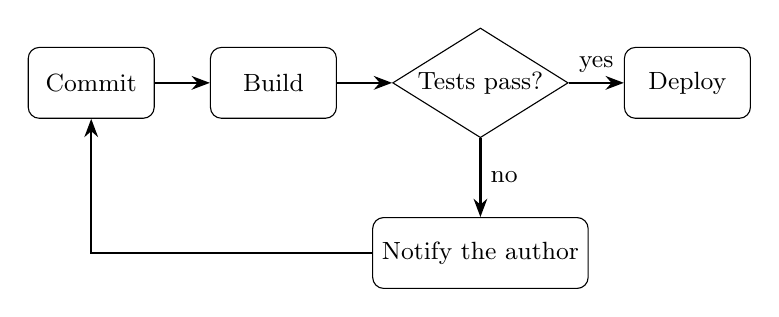
\begin{tikzpicture}[
  node distance=6mm and 7mm,
  every node/.style={font=\small},
  stage/.style={rectangle, rounded corners, draw, minimum height=9mm, minimum width=16mm},
  gate/.style={diamond, aspect=1.6, draw, inner sep=1pt},
  arrow/.style={-{Stealth}, thick},
]
  \node[stage] (commit) {Commit};
  \node[stage, right=of commit] (build) {Build};
  \node[gate, right=of build] (test) {Tests pass?};
  \node[stage, right=of test] (deploy) {Deploy};
  \node[stage, below=10mm of test] (notify) {Notify the author};

  \draw[arrow] (commit) -- (build);
  \draw[arrow] (build) -- (test);
  \draw[arrow] (test) -- node[above] {yes} (deploy);
  \draw[arrow] (test) -- node[right] {no} (notify);
  \draw[arrow] (notify) -| (commit);
\end{tikzpicture}
